\chapter{Material and method}
\label{chap:m&m}

\section{Material}

\subsection{Laboratory instruments}
BD Accuri C6 Plus benchtop flow cytometer (BD Nordics (prev. Puls Norway), Norway). Filters and lasers.
CytoSub submersible flow cytometer (CytoBuoy, Netherlands)
Coulter Counter Multisizer4 (Beckman Coulter, US) eqipped with a 100 \micro m aperature (size-range 2-60 \micro m)
Nikon Eclipse Ni-U Upright Microscope equipped with a CMOS camera (MC170HD, Leica Microsystems, Germany), [Filters: Nikon Brightline GFP-4050B filter-cube (channel 6), Objectives: Plan Fluor 40x/0.75 water immersion objective, Plan Fluor 100x/1.30 Oil immersion objective]
Leitz Labrolux 12 binocular microscope (Leica Mikroskopi AS, Norway) [EF 40/0.65 objective]
Eppendorf Centrifuge 5804 R (Eppendorf, Norway), [rotor: A-4-44, rotor radius: 15.5 cm], high-speed refrigerated benchtop centrifuge
Jouan KR22i floor centrifuge (Thermo Fischer Scientific, US), high-speed high capacity refrigerated floor centrifuge 8 [rotor: AK 100-21]
Bürker Counting Chamber (Hirschmann Laborgeräte, Germany) with 0.1 mm depth of chamber
Eirik Lund sitt kamera, lense og imaging software: 
Sony ILCE A6400 with E-mount, lense: Tamron 17-70mm F/2.8 
Adobe\textsuperscript{\textregistered} Lightroom Classic 12.0 

\begin{table}[H]
	\centering
	%\caption{Chemicals used in the master thesis, listed alphabetically according to chemical name, including the chemical's CAS nr., purity/grade, supplier and state.}
	\label{tb:instruments}
	\resizebox{\linewidth}{!}{
	\begin{tabular}{lll}
	\textbf{Instrument} & \textbf{Commercial name} & \textbf{Producer} \\
		\midrule
   Benchtop Flow Cytometer               & BD Accuri$^{TM}$ C6 Plus & BD Biosciences \\
   Submersible Flow Cytometer            & Cytosub                  & CytoBuoy \\
   Coulter Counter                       & Multisizer 4             & Beckman Coulter \\
   Upright microscope                    & Eclipse Ni-U             & Nikon \\
   Transmitted/incident light microscope & Labrolux 12              & Leitz \\
   CMOS camera                           & MC170HD                  & Leica Microsystems \\
   Benchtop centrifuge                   & Centrifuge 5804 R        & Eppendorf\\
   Floor centrifuge                      & KR22i                    & Jouan \\
   Counting chamber                      & Bürker                   & Hirschmann \\
   		\bottomrule
	\end{tabular}
	}
\end{table}


\subsection{Chemicals}
\begin{table}[H]
	\centering
	%\caption{Chemicals used in the master thesis, listed alphabetically according to chemical name, including the chemical's CAS nr., purity/grade, supplier and state.}
	\label{tb:chemical-list}
	\resizebox{\linewidth}{!}{
	\begin{tabular}{lllll}
	\textbf{Chemicals (abbrv.)} & \textbf{CAS-nr.} & \textbf{Purity/grade} & \textbf{Supplier} & \textbf{state} \\
		\midrule
    D-(+)-Glucose                   & 50-99-7    & $\geq$ 99.5    & Sigma Aldrich & s \\
    EDTA anhydrous                  & 60-00-4    & $\geq$ 99 \%   & Sigma Aldrich & s \\
    \ce{Na2EDTA}$\cdot$\ce{2H2O}    & 6381-92-6  & 98.5-101.5 \%  & Sigma Aldrich & s \\
    Ethanol                         & 64-17-5    & 96 \% vol      & VWR           & l \\
    Sodium chloride                 & 7647-14-5  & $\geq$ 99.5 \% & Merck         & s \\
    Dimethyl sulfoxide              & 67-68-5    & $\geq$ 99.5 \% & Sigma Aldrich & l \\
    Methanol                        & 67-56-1    & $\geq$ 99.9 \% & Sigma Aldrich & l \\
    Tris(hydroxymethyl)aminomethane & 77-86-1    & ACS reagent    & Merck         & s \\
    
		\bottomrule
	\end{tabular}
	}
\end{table}


\subsection{Reagents for Flow Cytometry}
\begin{table}[H]
	\centering
	%\caption{Reagents and kits used in the master thesis, listed alphabetically according to product name, including manufacturer, supplier and supplier's catalogue number.}
	\label{tb:reagent-list}
	\resizebox{\linewidth}{!}{
	\begin{tabular}{lllll}
	\textbf{Product name (abbrv.)} & \textbf{Manufacturer} & \textbf{Supplier} & \textbf{Catalogue} & \textbf{Dilution} \\
		\midrule
    TO-PRO-3 &  InVitrogen$^{TM}$  & Thermo Fisher	& T3605 & 1:20 \\
    Ethidium Homodimer-1 &  InVitrogen$^{TM}$ & Thermo Fisher &  E1169 & 4 \micro L/sample \\
    Apotracker$^{TM}$ Green & BioLegend & Fisher Scientific & 50-207-9934 & NA \\
    Calcein-AM & Invitrogen$^{TM}$ & Thermo Fisher & C1430 & 1:80 \\ 
    CS\&T RUO beads & BD Biosciences & BD Biosciences & 661414 &  4 drops/mL \\
    8-peak validation beads & Spherotech & BD Biosciences & 653144 & 4 drops/mL \\
    6-peak validation beads & Spherotech & BD Biosciences & 653145 & 4 drops/mL \\
		\bottomrule
	\end{tabular}
	}
\end{table}


\subsection{Microscopy kits and reagents}
\begin{table}[H]
	\centering
	%\caption{Reagents and kits used in the master thesis, listed alphabetically according to product name, including manufacturer, supplier and supplier's catalogue number.}
	\label{tb:Microscopy-list}
	\resizebox{\linewidth}{!}{
	\begin{tabular}{llll}
	\textbf{Product name (abbrv.)} & \textbf{Producer} & \textbf{Supplier} & \textbf{Catalogue} \\
		\midrule
    Giemsa's azur eosin methylene blue solution & Merck & Sigma Aldrich & 1.09204.0500 \\
    Hemacolor\textsuperscript{\textregistered} & Sigma Aldrich & Sigma Aldrich & 1.11661 \\
    Eukitt\textsuperscript{\textregistered} Quick-hardening mounting medium & Orsatec GmbH & Sigma Aldrich & 03989 \\
    Type N Immersion Oil for Microscopy & Nikon & ? & MXA20234 \\
    Methanol & Merck & Sigma Aldrich & 1.06009.2511 \\
    Percoll$^{TM}$ & Cytiva Sweden AB & Sigma Aldrich & GE17-0891-02 \\
    Centrifuge tubes, Oak Ridge, 50 mL & Nalgene\textsuperscript{\textregistered} & VWR & 525-0046 \\
		\bottomrule
	\end{tabular}
	}
\end{table}






\subsection{Buffers and solutions}
\begin{table}[H]
	\centering
	\label{tb:buffers}
	\resizebox{\linewidth}{!}{
	\begin{tabular}{ll}
	\textbf{Buffer} & \textbf{Composition} \\
		\midrule
    MAS                   &  375.6 mM \ce{NaCl}, 28.97 mM Citric Acid$\cdot$3Na$\cdot$2\ce{H2O}, 113.8 mM D-Glucose, \\ 
                          & 2.617 mM Citric Acid$\cdot$\ce{H2O}, 11.5 mM \ce{Na2EDTA}$\cdot$\ce{2H2O} \\
    Anticoagulant buffer  & 55.5 mM D-glucose, 171.1 mM NaCl, 13.43 mM \ce{Na2EDTA}$\cdot$\ce{2H2O}, \\
                          & 0.05 M TRIS/HCl, pH=7.6 \\ 
    PBS                                  & 136.9 mM \ce{NaCl}, 2.7 mM \ce{KCl}, 10.1 mM \ce{Na2HPO4}, 1.8 mM \ce{KH2PO4} \\
    Sorensen Buffer       & 66.67 mM \ce{KH2PO4}, 66.67 mM \ce{Na2HPO4}$\cdot$\ce{2H2O}, pH=6.8 \\
    Leibovitz-15          &                                              \\
    HBSS                  &                                              \\
    Hemolymph solution    &                                              \\
		\bottomrule
	\end{tabular}
	}
\end{table}

\section{Method}
\subsection{Experimental setup/}
Mention M. edulis mean/median shell length, age (collected date/month/year), supplier (Snadder og Snaskum AS, Indre Fosen), transportation, that the supplier were asked not to shrub the shells, animal housing prior to experiment (erated, flow through volume, temperature, water type/source, time period, feeding, did they attach with byssus?), decribe depuration period

\subsection{Hemolymph extraction/Extraction of hemolymph/Hemolymph sampling technique}
To minimize the possibility of contaminating hemolymph samples during extraction, a simple and time-effective sampling technique modified from the nonlethal technique of Gustafson et al., 2005 was developed. The method was centered around achieving good visual contact with the posterior adductor muscle and the position of the needle within the muscle during hemolymph withdrawal, and were mainly constricted by the requirement of an intact digestive gland.

In order to access and see the posterior adductor muscle while staying clear of the digestive gland, the valves were prised apart ventrally by gently forcing a tissue forceps between the valves ventromedially (Fig. \ref{fig:Hemolymph_sampling_illustration}a). Since the posterior adductor muscle is oblong in the anteroposterior direction, penetrating the muscle from the posterior end pointing straight anteriorly gave the operator better margins to avoid piercing the muscle. To create a free path to the muscle from the posterior direction, the mantle immediately surrounding the inhalant and exhalant syphon where cut with a scalpel (Fig. \ref{fig:Hemolymph_sampling_illustration}b and d), holding the blunt spine of the scalpel blade facing the posterior adductor muscle.  Thus, when illuminating the interior of the mussel from above with the ventral aspect facing upwards, the operator is able to supervise the position of the needle in the muscle sinus trough the slightly transparent posterior adductor muscle, as seen in Fig. \ref{fig:Hemolymph_sampling_illustration}c. The mussels were placed in the palm of the operator's non-dominant arm, 3$^{rd}$-5$^{th}$ digits firmly gripping the mussel, first and second digits holding the syringe steady in the anteroposterior direction, while the dominant arm were used to withdraw the syringe plunger.

Using the method described above, Technicalities of the withdrawal (1 mL syringes with 27 gauche needles), syringe filled with 0.5 mL anticoagulant solution (MAS or the one from Pipe, 1997). Volume withdrawn, dilution to 1:1 hemolymph:MAS is volume > 0.5 mL hemolymph was withdrawn.


\begin{figure}
    \centering
    \begin{subfigure}[b]{.45\textwidth}
        \centering
        \includegraphics[width=\textwidth]{figures/Sampling technique/forceps square color.jpg}
        \caption{Placement of forceps between valves on the ventral side of the mussel.}
        \label{sfig:a}
    \end{subfigure}
    \hfill
    \begin{subfigure}[b]{.45\textwidth}
        \centering
        \includegraphics[width=\textwidth]{figures/Sampling technique/uncut color 3495.jpg}
        \caption{Posterior aspect of mussel with the mantle (red arrow) intact.}
        \label{sfig:b}
    \end{subfigure}
    \newline
    \begin{subfigure}[b]{.45\textwidth}
        \centering
        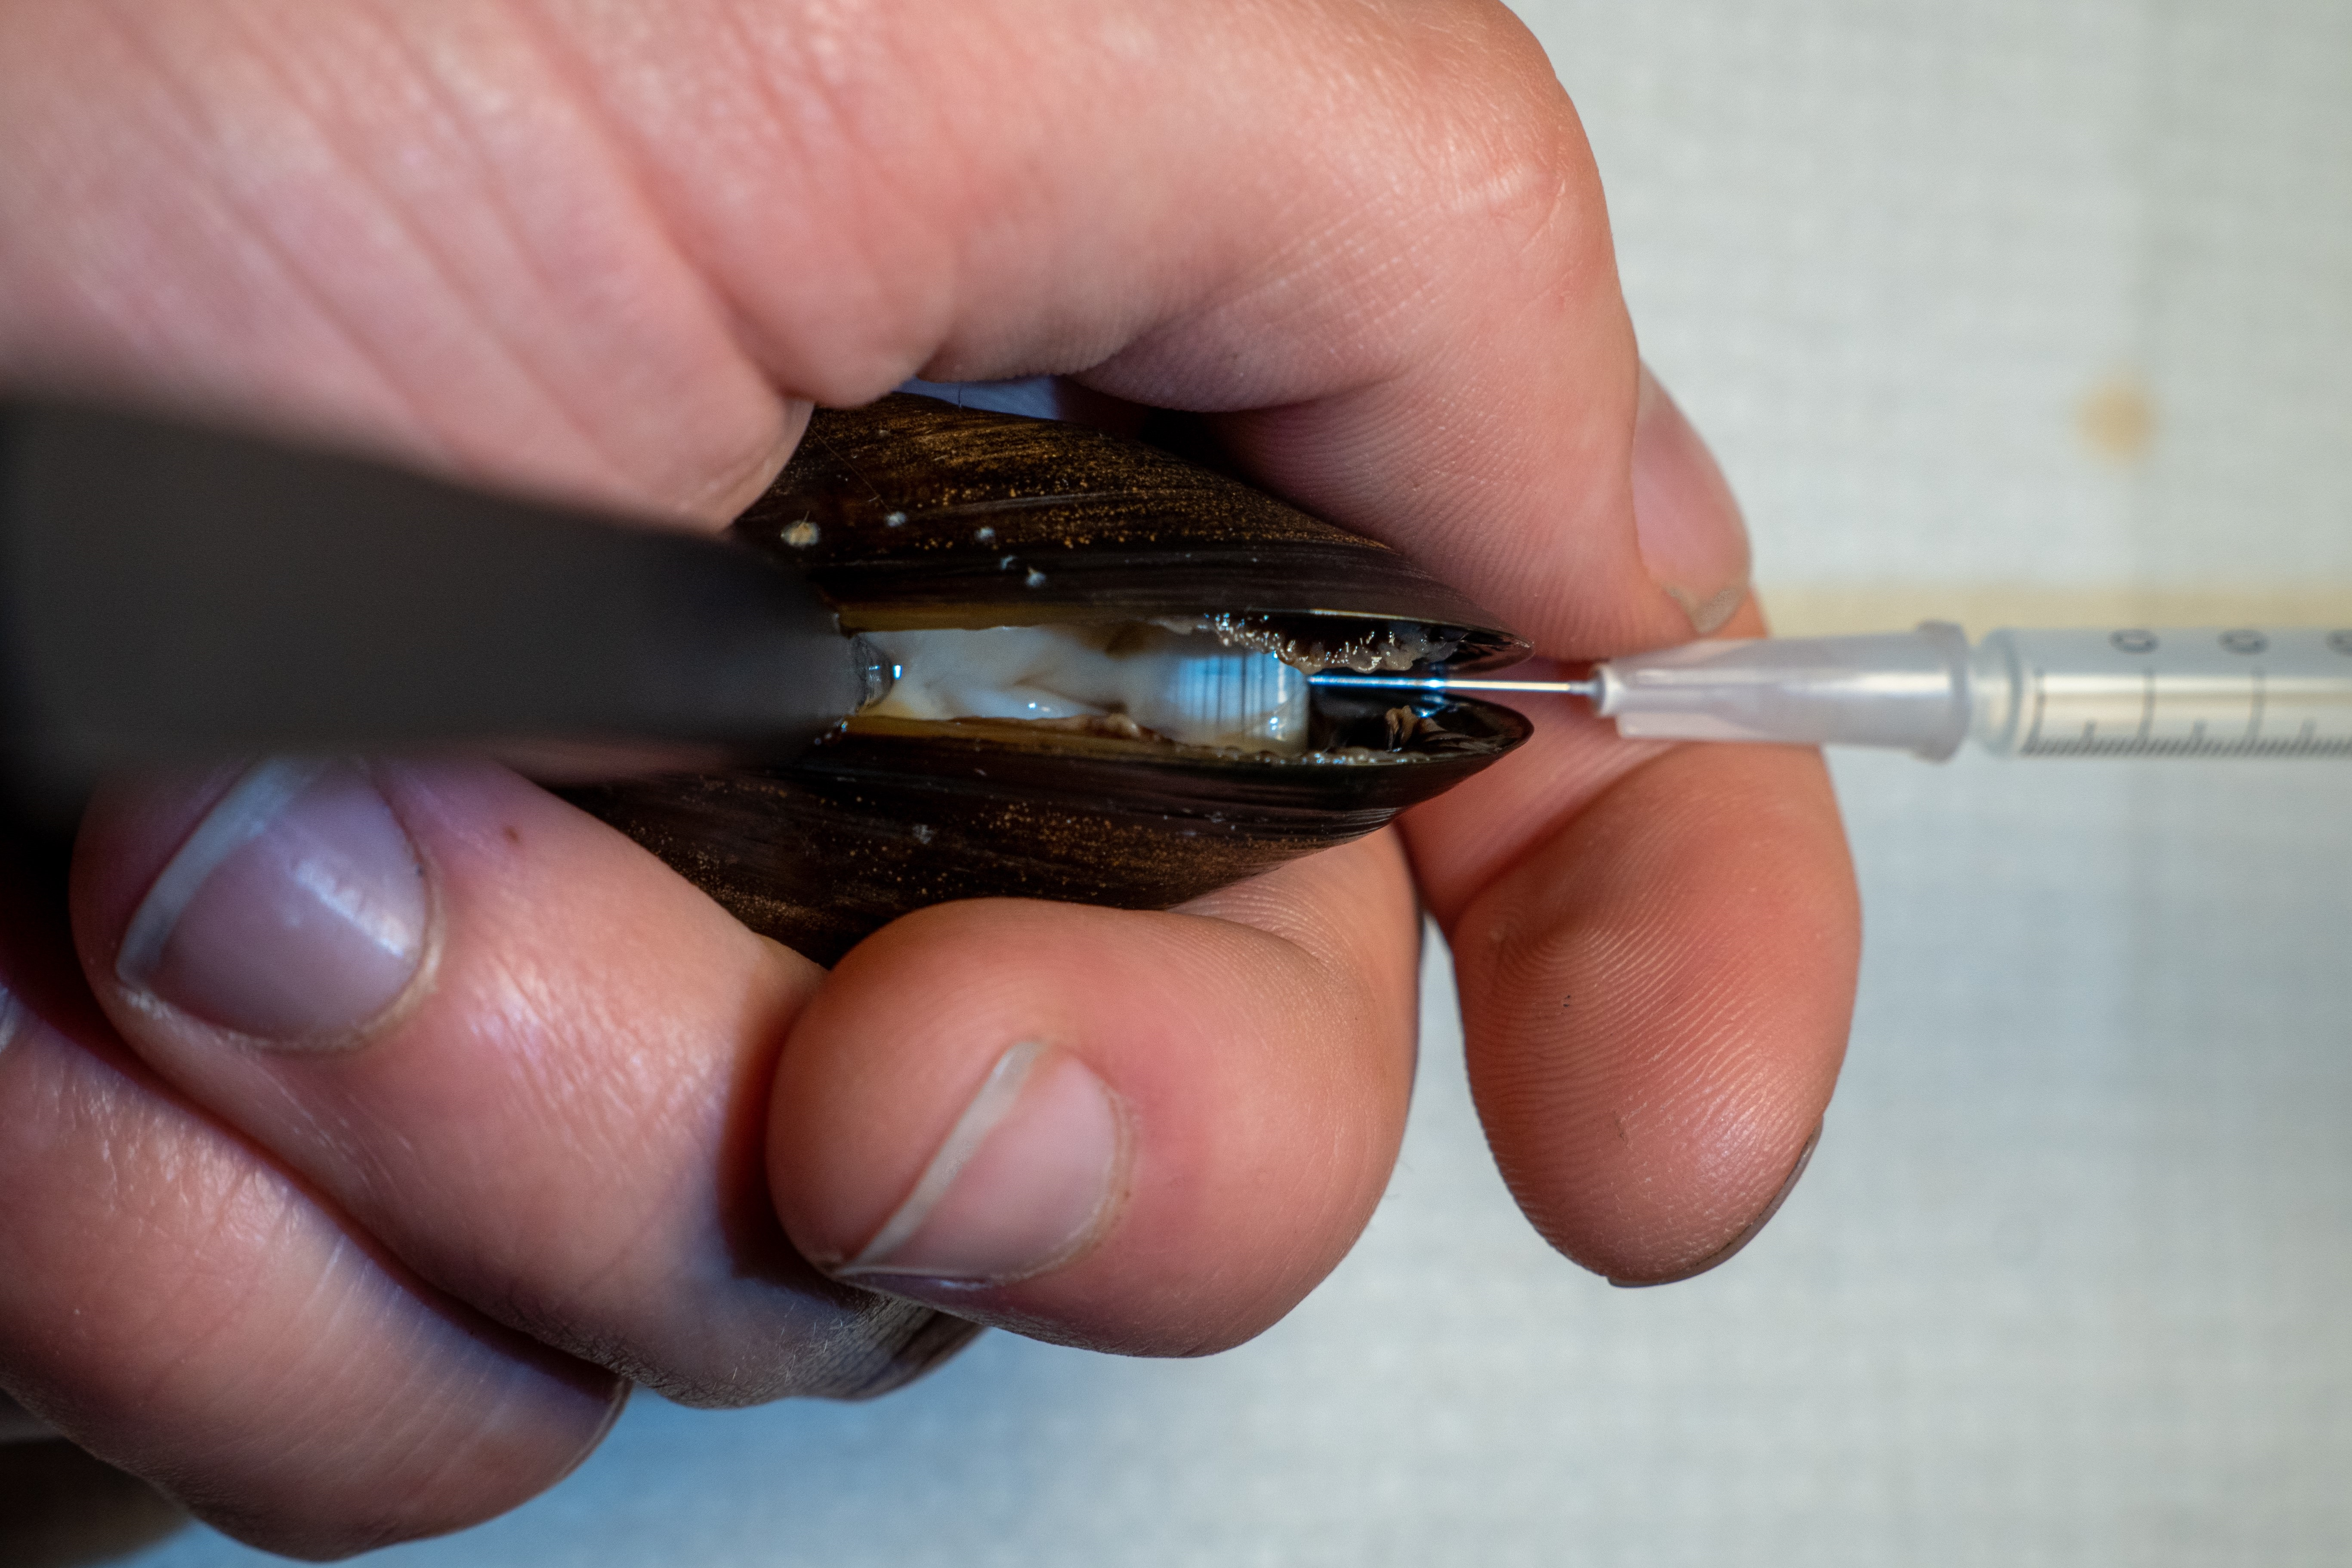
\includegraphics[width=\textwidth]{figures/Sampling technique/hands colors centered.jpg}
        \caption{The mussel grip and needle alignment employed, seen from the operators perspective. }
        \label{sfig:c}
    \end{subfigure}
    \hfill
    \begin{subfigure}[b]{.45\textwidth}
        \centering
        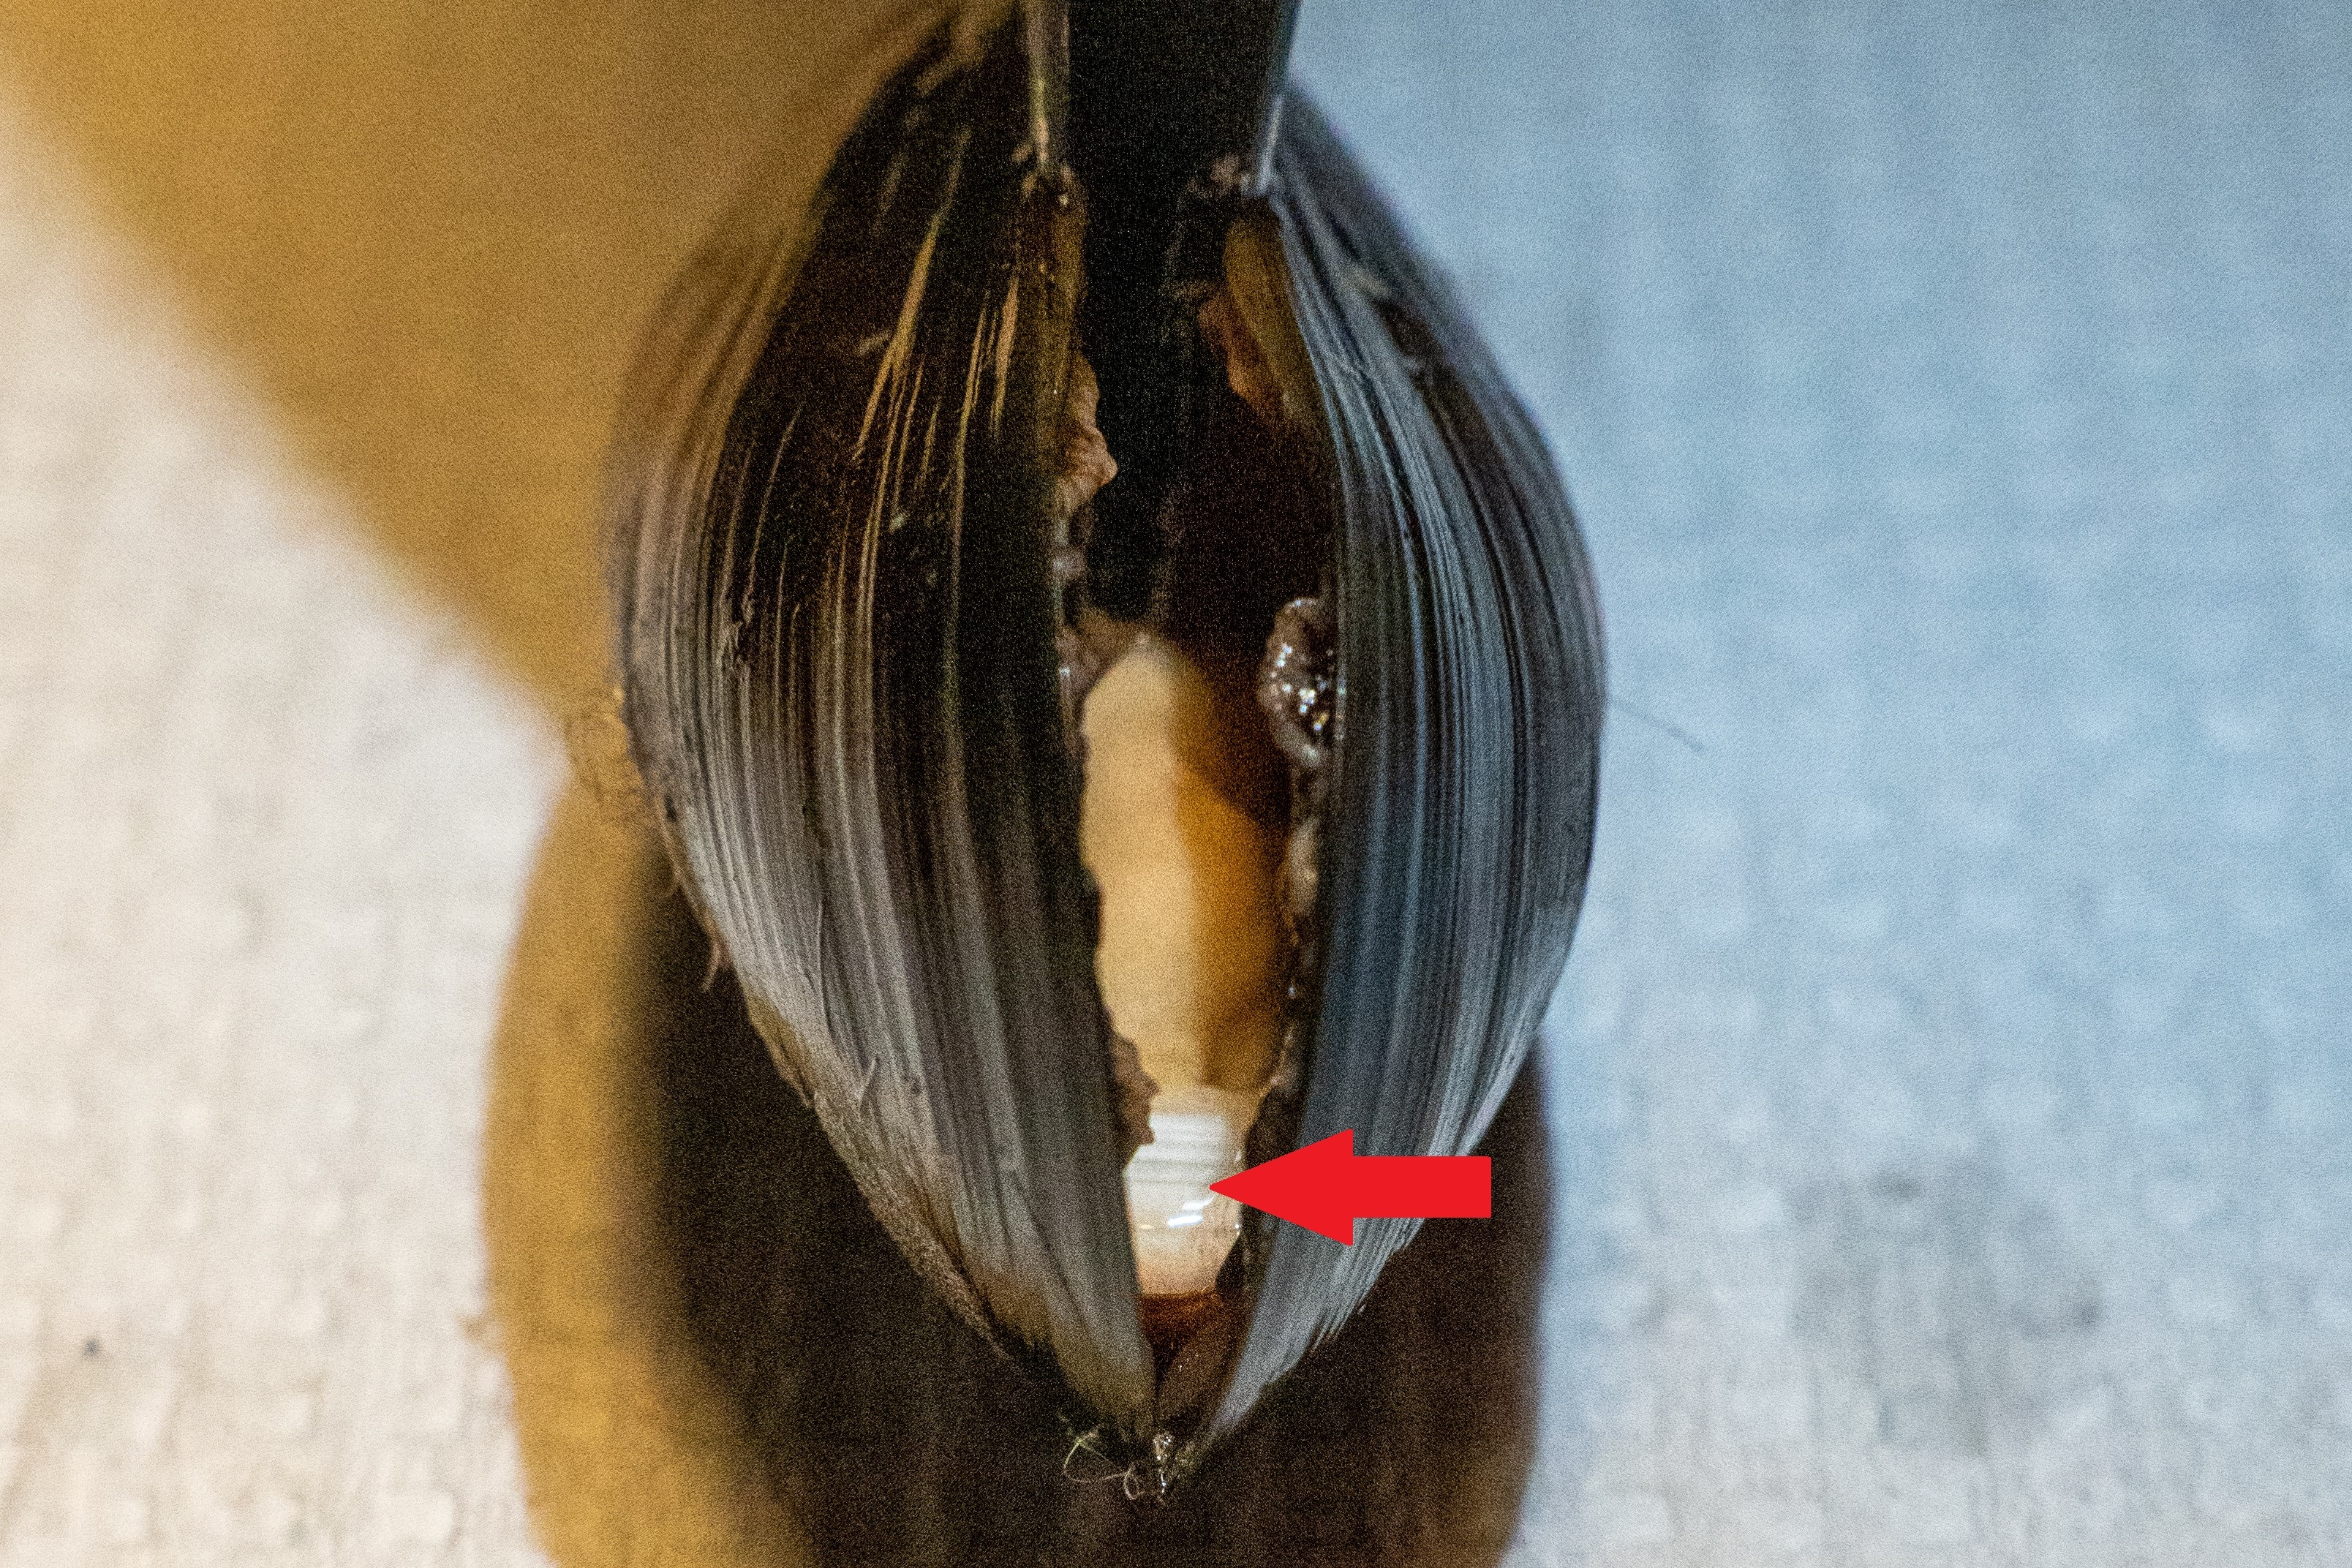
\includegraphics[width=\textwidth]{figures/Sampling technique/possible match.jpg}
        \caption{Mussel with visible posterior adductor muscle (red arrow) where the mantel was cut.}
        \label{sfig:d}
    \end{subfigure}
    \caption{An illustration of the method employed to extract hemolymph from M. edulis in order to avoid off-target withdrawal of fluid from surrounding tissues or enclosed seawater.}
    \label{fig:Hemolymph_sampling_illustration}
\end{figure}


What mean purity of hemocytes was obtained from the hemolymph sampling technique employed? Use the \% of plot in hemocyte gate from all samples run on flow cytometer before or during (or both) sampling period.

Adobe\textsuperscript{\textregistered} Lightroom Classic 12.0 
Sony ILCE A6400 with E-mount, lense:  